%% ============================================================================
%% fig_2_1_clam_tr_architecture.tex -- TikZ source of thesis Figure 7 (label
%% fig:clamtr_architecture, Ch.2 Section "CLAM-TR Architecture"). Adapted from
%% panel (a) of the architecture figure of the companion journal paper, in the
%% notation of the thesis (n, T, I, H_I, C_I, D_enc, M_clam, M_ret).
%% Every element follows the thesis text and the v20 code (cells 6, 10, 11, 19,
%% 21, 23, 25 of 04-final-v20/CLAM_TR_v20_UNI_Colab.ipynb):
%%   - feature transform Linear(D_enc, 512) -> ReLU -> Dropout BEFORE attention/TopK;
%%   - gated attention scores all N patches (temperature T); softmax over all N;
%%     TopK = min(128, N) by score; CLAM branch uses the NON-renormalised weights;
%%   - retention branch: configuration-dependent module on H_I, then the mean over
%%     the K selected patches; coordinates C_I only for the spatial-decay heads;
%%   - ADDITIVE fusion M_clam + M_ret -> Linear(512, 6); nothing in between.
%%
%% Sizes (KTU thesis guide, section 5.1: figure text >= 10 pt), laid out for 10 pt
%% text at scale 1: \footnotesize = 10.5 pt (titles, main formulas), \scriptsize =
%% 10.05 pt (details, arrow labels); math sub/superscripts 7.04 pt (the script size
%% of 10 pt text, the guide's exception).
%% Inline fractions use \dfrac so that 1 and K print at text size.
%% Layout: the trunk is a column (top to bottom) on the left, the configuration key
%% top right, the two branches, the fusion and the classifier bottom right.
%% Natural width = \textwidth (15.5 cm): include with width=\textwidth (scale ~1).
%% ============================================================================
\documentclass[border=1pt]{standalone}
\usepackage[T1]{fontenc}
\usepackage{amsmath}
\usepackage{newtxtext,newtxmath}
\usepackage{tikz}
\usetikzlibrary{arrows.meta,calc,positioning}

%% ---- every non-script text item >= 10 pt at printed size ---------------------------------------------------
\makeatletter
\renewcommand\footnotesize{\@setfontsize\footnotesize{10.5}{12.6}}
\renewcommand\scriptsize{\@setfontsize\scriptsize{10.05}{12.1}}
\makeatother
\DeclareMathSizes{10}{10}{7.04}{7.04}
\DeclareMathSizes{10.05}{10.05}{7.04}{7.04}
\DeclareMathSizes{10.5}{10.5}{7.35}{7.04}
\hyphenpenalty=10000
\exhyphenpenalty=10000
%% -------------------------------------------------------------------------------------------------------------
\begin{document}
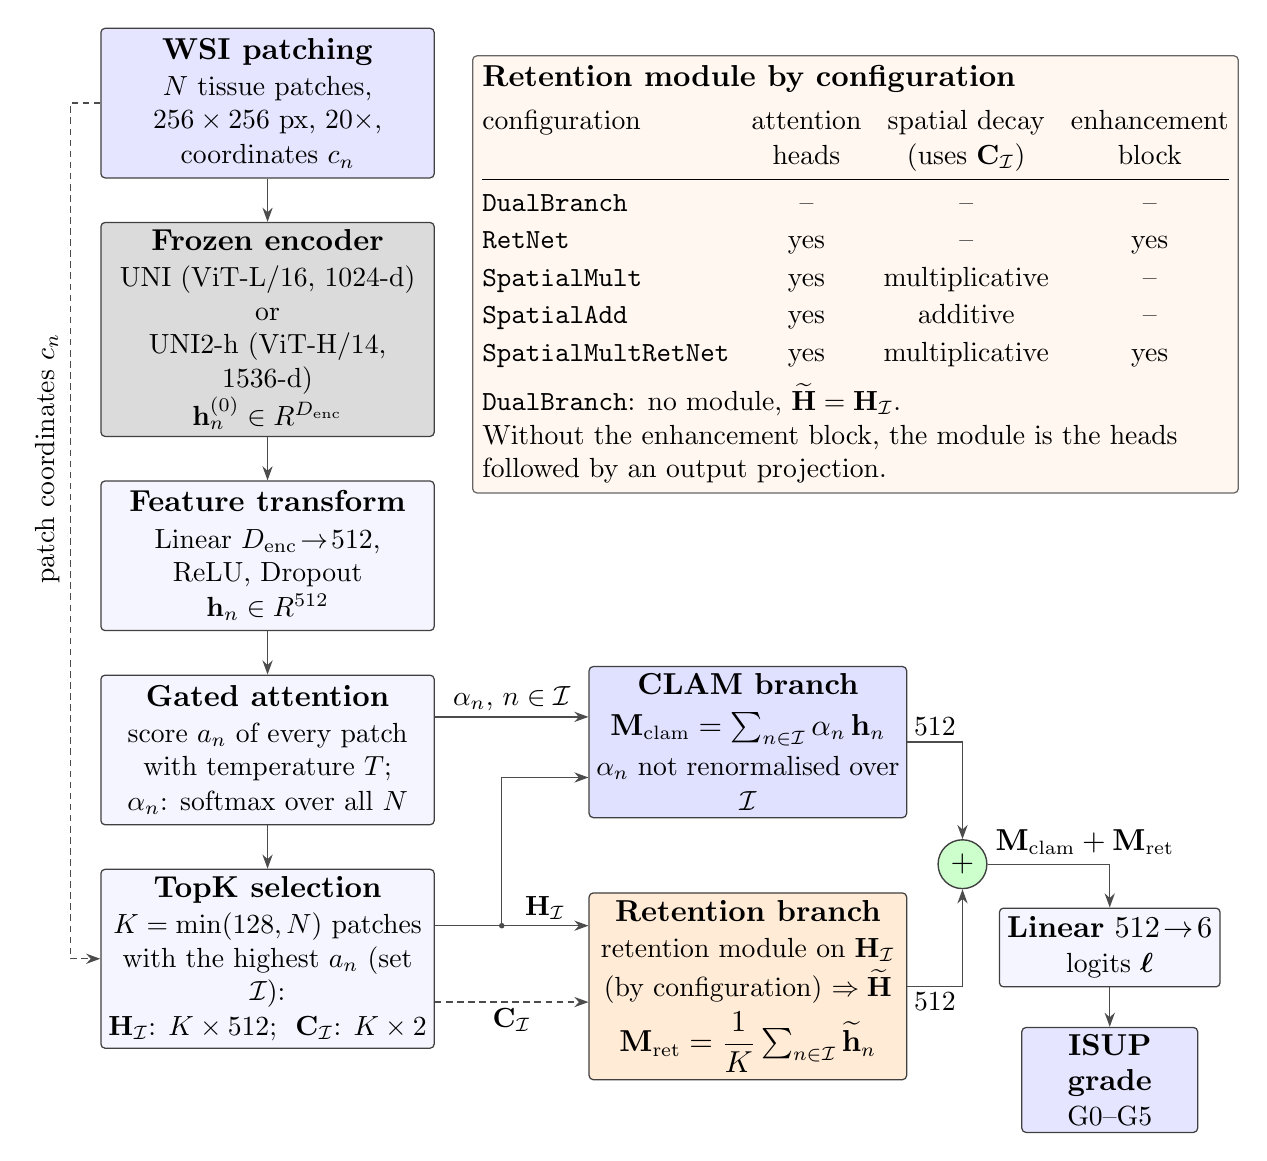
\begin{tikzpicture}[
  font=\footnotesize,
  >={Stealth[length=1.8mm,width=1.3mm]},
  base/.style={draw=black!75, rounded corners=1.5pt, line width=0.45pt,
               align=flush center, inner sep=2.6pt},
  trunk/.style={base, inner sep=2.6pt, fill=blue!4, text width=4.05cm, minimum height=19mm},
  frozen/.style={trunk, fill=black!14},
  io/.style={trunk, fill=blue!10},
  clam/.style={base, fill=blue!12, minimum height=17mm},
  ret/.style={base, fill=orange!16, minimum height=17mm},
  sm/.style={draw=black!75, circle, minimum size=6.2mm, inner sep=0pt, fill=green!20,
             line width=0.5pt, font=\footnotesize},
  small/.style={base, minimum height=10mm},
  ar/.style={->, line width=0.5pt, draw=black!70},
  dar/.style={->, line width=0.5pt, draw=black!70, dash pattern=on 2.4pt off 1.6pt},
  lab/.style={font=\scriptsize, inner sep=1pt}
]

% ---------------------------- shared trunk (one column, top to bottom) -------
\node[io, anchor=north west] (a1) at (0.80,0)
  {\textbf{WSI patching}\\[1pt]
   {\scriptsize $N$ tissue patches,\\ $256\times256$ px, $20\times$,\\ coordinates $c_{n}$}};
\node[frozen, below=5.5mm of a1] (a2)
  {\textbf{Frozen encoder}\\[1pt]
   {\scriptsize UNI (ViT-L/16, 1024-d) or\\ UNI2-h (ViT-H/14, 1536-d)\\
    $\mathbf{h}^{(0)}_{n}\in\mathbb{R}^{D_{\mathrm{enc}}}$}};
\node[trunk, below=5.5mm of a2] (a3)
  {\textbf{Feature transform}\\[1pt]
   {\scriptsize Linear $D_{\mathrm{enc}}\!\rightarrow\!512$,\\ ReLU, Dropout\\
    $\mathbf{h}_{n}\in\mathbb{R}^{512}$}};
\node[trunk, below=5.5mm of a3] (a4)
  {\textbf{Gated attention}\\[1pt]
   {\scriptsize score $a_{n}$ of every patch\\ with temperature $T$;\\
    $\alpha_{n}$: softmax over all $N$}};
\node[trunk, below=5.5mm of a4, minimum height=21mm] (a5)
  {\textbf{TopK selection}\\[1pt]
   {\scriptsize $K=\min(128,N)$ patches\\ with the highest $a_{n}$ (set $\mathcal{I}$):\\
    $\mathbf{H}_{\mathcal{I}}$: $K\times512$; \ $\mathbf{C}_{\mathcal{I}}$: $K\times2$}};
\foreach \u/\v in {a1/a2, a2/a3, a3/a4, a4/a5} \draw[ar] (\u) -- (\v);

% patch coordinates bypass encoder, transform and attention; selected at TopK
\draw[dar] (a1.west) -- (0.42,0 |- a1.west) -- (0.42,0 |- a5.west) -- (a5.west);
\node[lab, rotate=90, anchor=south, inner sep=2.6pt] at ($(0.42,0 |- a2.south)!0.5!(0.42,0 |- a3.north)+(-0.04,0)$)
  {patch coordinates $c_{n}$};

% ---------------------------- two branches (right of gated attention / TopK) --
\node[clam, anchor=west, text width=3.85cm] (b1) at ($(7.00,0 |- a4.center)+(0,0.10)$)
  {\textbf{CLAM branch}\\[2pt]
   $\mathbf{M}_{\mathrm{clam}}=\sum_{n\in\mathcal{I}}\alpha_{n}\,\mathbf{h}_{n}$\\[2pt]
   {\scriptsize $\alpha_{n}$ not renormalised over $\mathcal{I}$}};
\node[ret, anchor=west, text width=3.85cm] (b2) at ($(7.00,0 |- a5.center)+(0,-0.35)$)
  {\textbf{Retention branch}\\[1pt]
   {\scriptsize retention module on $\mathbf{H}_{\mathcal{I}}$\\[1.5pt] (by configuration)
    $\Rightarrow\widetilde{\mathbf{H}}$}\\[2pt]
   $\mathbf{M}_{\mathrm{ret}}=\dfrac{1}{K}\sum_{n\in\mathcal{I}}\widetilde{\mathbf{h}}_{n}$};

% weights alpha_n (softmax over all N) enter the CLAM branch for n in I
\draw[ar] ($(a4.east)+(0,0.42)$) -- ($(b1.west |- a4.east)+(0,0.42)$)
  node[lab, midway, above=1pt] {$\alpha_{n}$, $n\in\mathcal{I}$};
% selected features to both branches
\coordinate (hI) at ($(a5.east)+(0,0.42)$);
\coordinate (fork) at ($(hI)+(0.85,0)$);
\draw[line width=0.5pt, draw=black!70] (hI) -- (fork);
\fill[black!70] (fork) circle (1.0pt);
\draw[ar] (fork) |- ($(b1.west)+(0,-0.45)$);
\draw[ar] (fork) -- (fork -| b2.west);
\node[lab, anchor=south] at ($(fork)!0.5!(fork -| b2.west)+(0,0.03)$)
  {$\mathbf{H}_{\mathcal{I}}$};
% coordinates only towards the retention branch
\draw[dar] ($(a5.east)+(0,-0.55)$) -- ($(b2.west |- a5.east)+(0,-0.55)$)
  node[lab, midway, below=1pt] {$\mathbf{C}_{\mathcal{I}}$};

% ---------------------------- fusion and classifier -------------------------
\coordinate (xs) at (11.75,0);
\path (xs |- b1.east) coordinate (s1);
\path (xs |- b2.east) coordinate (s2);
\node[sm] (sum) at ($(s1)!0.5!(s2)$) {$+$};
\draw[ar] (b1.east) -- node[lab, above=1pt] {512} (s1) -- (sum.north);
\draw[ar] (b2.east) -- node[lab, below=1pt] {512} (s2) -- (sum.south);
\node[anchor=south west, inner sep=1pt] at ($(sum.east)+(0.06,0.08)$)
  {$\mathbf{M}_{\mathrm{clam}}+\mathbf{M}_{\mathrm{ret}}$};
\node[small, fill=blue!4, anchor=north, text width=2.62cm] (cls) at ($(13.62,0 |- sum.east)+(0,-0.55)$)
  {\textbf{Linear} $512\!\rightarrow\!6$\\[0pt] {\scriptsize logits $\boldsymbol{\ell}$}};
\node[small, fill=blue!10, anchor=north, text width=2.05cm] (out) at ($(cls.south)+(0,-0.50)$)
  {\textbf{ISUP grade}\\[0pt] {\scriptsize G0--G5}};
\draw[ar] (sum.east) -| (cls.north);
\draw[ar] (cls) -- (out);

% ---------------------------- configuration key (top right) -----------------
\node[draw=black!60, rounded corners=1.5pt, line width=0.45pt, fill=orange!6,
      anchor=north east, inner sep=3.5pt, font=\scriptsize, align=left] (key)
      at (15.26,-0.35)
  {{\footnotesize\textbf{Retention module by configuration}}\\[3pt]
   \renewcommand{\arraystretch}{1.12}%
   \begin{tabular}{@{}l@{\hspace{8pt}}c@{\hspace{8pt}}c@{\hspace{8pt}}c@{}}
     configuration & attention & spatial decay & enhancement \\[-1pt]
                   & heads     & (uses $\mathbf{C}_{\mathcal{I}}$) & block \\[1pt]
     \hline\noalign{\vskip 2pt}
     \texttt{DualBranch}        & --  & --              & --  \\
     \texttt{RetNet}            & yes & --              & yes \\
     \texttt{SpatialMult}       & yes & multiplicative  & --  \\
     \texttt{SpatialAdd}        & yes & additive        & --  \\
     \texttt{SpatialMultRetNet} & yes & multiplicative  & yes \\
   \end{tabular}\\[3pt]
   \texttt{DualBranch}: no module, $\widetilde{\mathbf{H}}=\mathbf{H}_{\mathcal{I}}$.\\
   Without the enhancement block, the module is the heads\\ followed by an output projection.};

\end{tikzpicture}
\end{document}
